\section{Knowledge base generator}
\begin{figure}[htp]
\centering
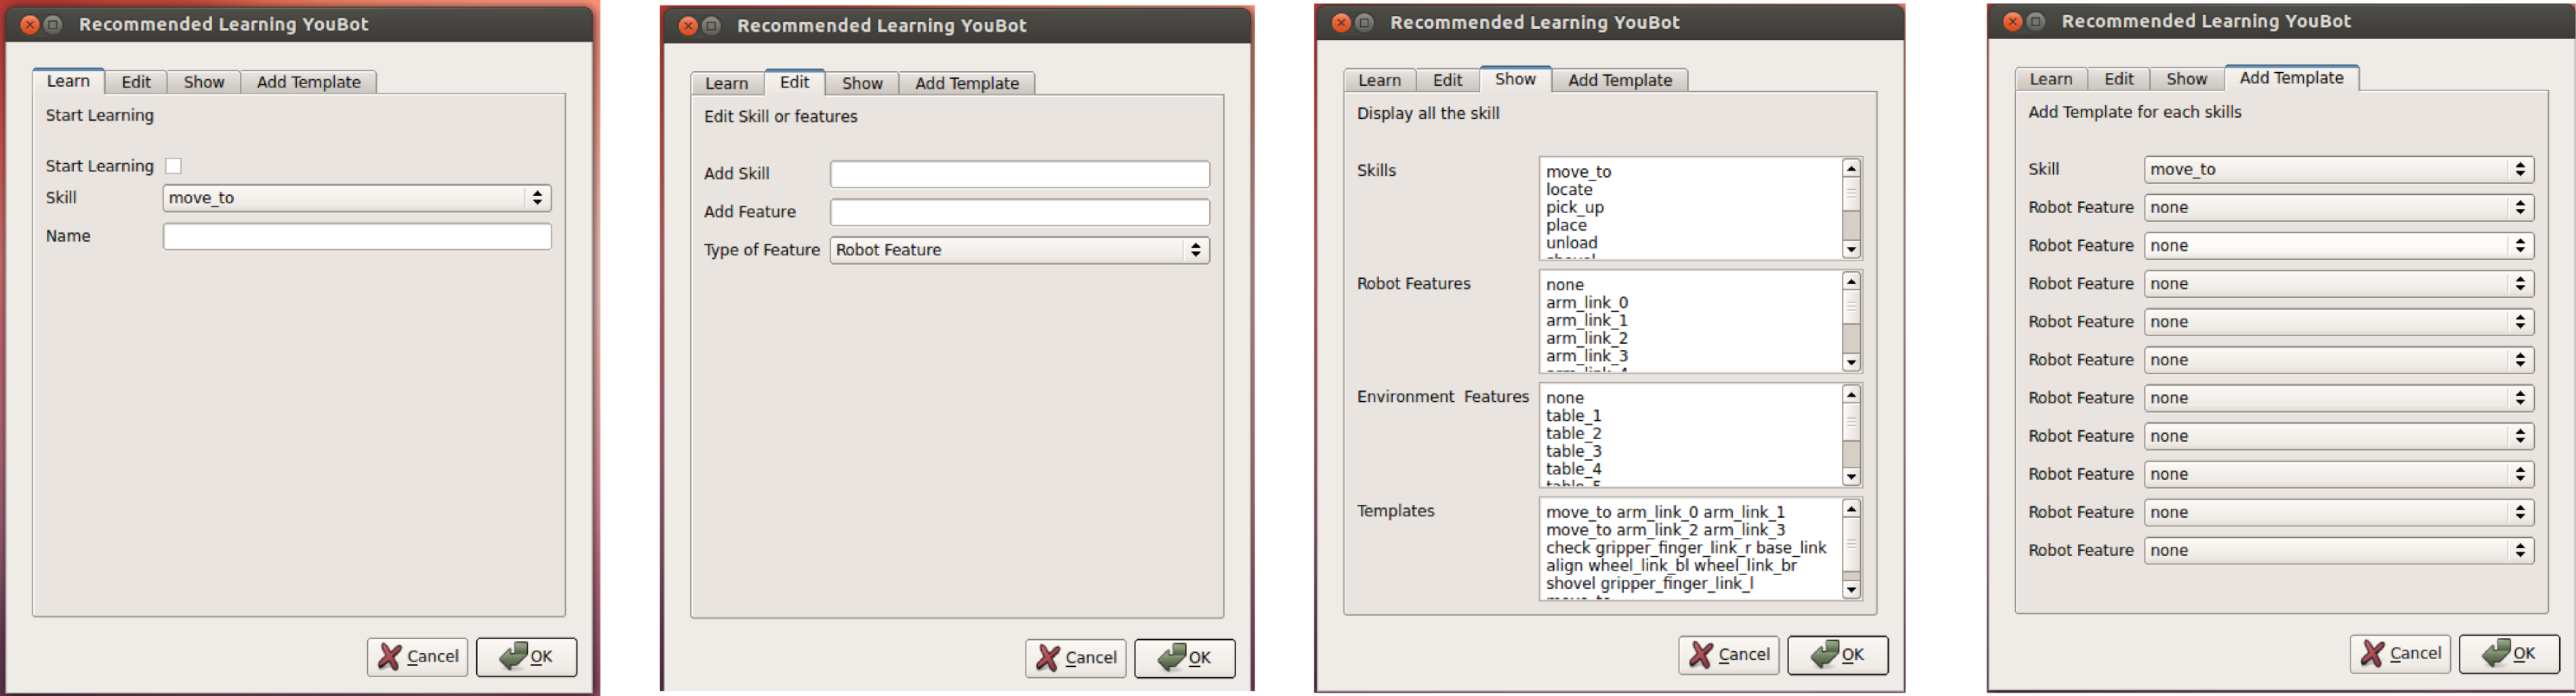
\includegraphics[scale=0.5]{images/tool/tool.png}
\caption[Tool for generating knowledge base]{Tool for generating knowledge base. 1) window for learning a new skill
2) window for editing skill or features 3) Display all features, skills and
templates 4) adding new templates}
\label{}
\end{figure}

On of the limitations of the current efforts in LfD is adding new features for
new task \cite {argall_survey_2009}. Due to the intuitive nature of
demonstration, LfD algorithms have the potential to make robot programming
accessible for everyday users who have no programming experience and want to
customize robot behaviours. The use of current approaches by the researchers
, however, is likely to lead to situations in which users attempt to
teach the robot tasks that cannot be learned simply due to the lack of features
describing some aspect of the task.

The solution to such an attempt would be have good tool where the user on 
identification of new features can add new features to the system on which 
the robot can learn.

Also the template creation is an actively changing scenario with various permutations
and combinations possible. The above mentioned tool can be used for rapid 
generation and modification of the templates.



\section{Use of Recommender system in robotics}
\subsection{Preferences of users in Task Planing}
\subsection{Kernel Recommendation in SVM}
Firstly, linearity is rather special, and outside quantum mechanics no
      model of a real system is truly linear. Secondly, detecting linear
relations has been the focus of much research in statistics and machine
learning for decades and the resulting algorithms are well understood, well
developed and efficient. Naturally, one wants the best of both worlds. So, if a
problem is non-linear, instead of trying to fit a non-linear model, one can map
the problem from the input space to a new (higher-dimensional) space (called
the feature space) by doing a non-linear transformation using suitably chosen
basis functions and then use a linear model in the feature space. This is known
as the 'kernel trick'. The linear model in the feature space corresponds to a
non-linear model in the input space. This approach can be used in both
classification and regression problems. The choice of kernel function is
crucial for the success of all kernel algorithms because the kernel constitutes
prior knowledge that is available about a task. Accordingly, there is no free
lunch (see No Free Lunch Theorems) in kernel choice.\footnote{\url{http://www.svms.org/kernels/}}
    * Recommender system : Collabrative Filter based can be used to determine 
which algo to use.

\subsection{Motion Path Planning algo in Planning }
     OMPL has implemented the following planners
      \url{http://ompl.kavrakilab.org/planners.html}
     Which planner to select can be done automatically explained here 
        "How OMPL selects a control-based planner?"
If you use the ompl control SimpleSetup class (highly recommended) to define
and solve your motion planning problem, then OMPL will automatically select an
appropriate planner (unless you have explicitly specified one). If the state
space has a default projection (which is going to be the case if you use any of
the built-in state spaces), then it will use KPIECE. This planner has been
shown to work well consistently across many real-world motion planning
problems, which is why it is the default choice. In case the state space has no
default projection, RRT will be used. Note that there are no bidirectional
control-based planners, since we do not assume that there is a steering
function that can connect two states exactly."
     Again Recommender Collabrative filter can be used to decide which algo to
      be used for recommendation.

\section{Softwares and tools}

A software implementation and number of tools have been included in the attached
$CD\-ROM$. The tools and the software developed as part of the project.
Below is a brief description of the packages

\begin{itemize}

    \item \textbf{Recommender Learning} \\
        Python based implementation of the learning approach. The class has to be 
        invoked with the folder containing the JSON file of the demonstrations.
        The JSON file is read and learning is made on base of the demonstrations.
        It also reads the knowledge base and creates the set of templates.
        It implements the approach mentioned in section \ref{sec:Learning motion primitive}.
        Available online : \url{https://github.com/deebuls/RecommenderSystemInRobotics/tree/master/code/recommended\_learning}

    \item \textbf{mir\_teleop\_record} \\
        ROS node for teleoperation of the youbot arm and the base. The node was 
        an extension of the work of b-it bots team \url{https://github.com/mas-group/robocup-at-work/tree/brazil-2014/mas\_common\_robotics/mcr\_tools/mcr\_teleop}.
        The node was modified to record the features and to create a JSON file with the readings.
        Available online : \url {https://github.com/deebuls/RecommenderSystemInRobotics/tree/master/code/mir\_teleop\_record }

    \item \textbf{Data accumulator} \\
        The python script for accumulating all the recorded json file and creating
        a consolidated JSON file of the demonstration.
        Available online : \url{https://github.com/deebuls/RecommenderSystemInRobotics/tree/master/code/tools }

    \item \textbf{Knowledge base creator} \\
        An interactive online tool for creating of the knowledge base.
        Menu driven GUI for active interaction with the user and easy to use
        template creation for the knowledge base.
        Available online : \url{ https://github.com/deebuls/RecommenderSystemInRobotics/tree/master/code/knowledge\_base\_creator}

\end{itemize}
